% =================================================================================================
% File:			desc_dp.tex
% Description:	Definisce la sezione relativa all'appendice sui design pattern
% Created:		2015-03-27
% Author:		Tesser Paolo
% Email:		tesser.paolo@mashup-unipd.it
% =================================================================================================
% Modification History:
% Version		Modifier Date		Change											Author
% 0.0.1 		2015-03-27 			creato scheletro								Tesser Paolo
% =================================================================================================
%
% =================================================================================================
%

% CONTENUTO DEL CAPITOLO



\section{Descrizione Design Pattern} % (fold)
\label{sec:descdp}
	\subsection{Design pattern architetturali} % (fold)

		\subsubsection{MVC} % (fold)

		\begin{figure}[htbp]
			\centering
			\centerline{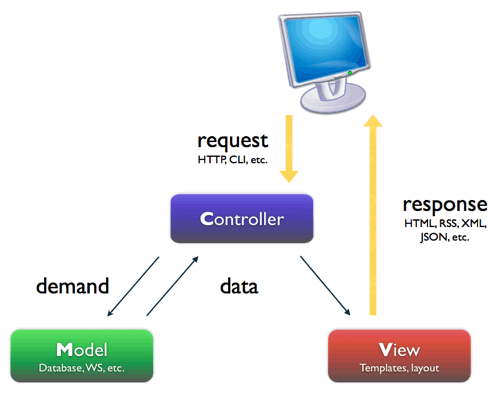
\includegraphics[scale=0.6]{./images/mvc.png}}
			\caption{Design pattern architetturale - MVC}
		\end{figure}

		Il pattern è basato sulla separazione dei compiti fra i componenti software che interpretano tre ruoli principali:
		\begin{itemize}
			\item \textbf{Model} che fornisce i metodi per accedere ai dati utili all'applicazione;
			\item \textbf{View} che visualizza i dati contenuti nel model e si occupa dell'interazione con utenti e agenti;
			\item \textbf{Controller} che riceve i comandi dell'utente (in genere attraverso il view) e li attua modificando lo stato degli altri due componenti.
		\end{itemize}
		\noindent
		Questo schema implica anche la tradizionale separazione fra la logica applicativa (in questo contesto spesso chiamata ``logica di business''), a carico del controller e del model, e l'interfaccia utente a carico del view. I dettagli delle interazioni fra questi tre oggetti software dipendono molto dalle tecnologie usate (linguaggio di programmazione, eventuali librerie, middleware e via dicendo) e dal tipo di applicazione (per esempio se si tratta di un'applicazione web, o di un'applicazione desktop). Quasi sempre la relazione fra view e model è descrivibile anche come istanza del pattern Observer. A volte, quando è necessario cambiare il comportamento standard dell'applicazione a seconda delle circostanze, il controller implementa anche il pattern Strategy.

		% subsubsection mvc (end)
	% subsection design_pattern_architetturali (end)



	\clearpage \newpage

	\subsection{Design pattern creazionali} % (fold)
	[TO DO]
	% subsection design_pattern_creazionali (end)

	\clearpage \newpage

	\subsection{Design pattern strutturali} % (fold)
	[TO DO]
	% subsection design_pattern_strutturali (end)

	\clearpage \newpage

	\subsection{Design pattern comportamentali} % (fold)
	[TO DO]
	% subsection design_pattern_comportamentali (end)


% section descdp (end)